\documentclass[12pt,a4paper]{article}\usepackage[]{graphicx}\usepackage[]{xcolor}
% maxwidth is the original width if it is less than linewidth
% otherwise use linewidth (to make sure the graphics do not exceed the margin)
\makeatletter
\def\maxwidth{ %
  \ifdim\Gin@nat@width>\linewidth
    \linewidth
  \else
    \Gin@nat@width
  \fi
}
\makeatother

\definecolor{fgcolor}{rgb}{0.345, 0.345, 0.345}
\newcommand{\hlnum}[1]{\textcolor[rgb]{0.686,0.059,0.569}{#1}}%
\newcommand{\hlsng}[1]{\textcolor[rgb]{0.192,0.494,0.8}{#1}}%
\newcommand{\hlcom}[1]{\textcolor[rgb]{0.678,0.584,0.686}{\textit{#1}}}%
\newcommand{\hlopt}[1]{\textcolor[rgb]{0,0,0}{#1}}%
\newcommand{\hldef}[1]{\textcolor[rgb]{0.345,0.345,0.345}{#1}}%
\newcommand{\hlkwa}[1]{\textcolor[rgb]{0.161,0.373,0.58}{\textbf{#1}}}%
\newcommand{\hlkwb}[1]{\textcolor[rgb]{0.69,0.353,0.396}{#1}}%
\newcommand{\hlkwc}[1]{\textcolor[rgb]{0.333,0.667,0.333}{#1}}%
\newcommand{\hlkwd}[1]{\textcolor[rgb]{0.737,0.353,0.396}{\textbf{#1}}}%
\let\hlipl\hlkwb

\usepackage{framed}
\makeatletter
\newenvironment{kframe}{%
 \def\at@end@of@kframe{}%
 \ifinner\ifhmode%
  \def\at@end@of@kframe{\end{minipage}}%
  \begin{minipage}{\columnwidth}%
 \fi\fi%
 \def\FrameCommand##1{\hskip\@totalleftmargin \hskip-\fboxsep
 \colorbox{shadecolor}{##1}\hskip-\fboxsep
     % There is no \\@totalrightmargin, so:
     \hskip-\linewidth \hskip-\@totalleftmargin \hskip\columnwidth}%
 \MakeFramed {\advance\hsize-\width
   \@totalleftmargin\z@ \linewidth\hsize
   \@setminipage}}%
 {\par\unskip\endMakeFramed%
 \at@end@of@kframe}
\makeatother

\definecolor{shadecolor}{rgb}{.97, .97, .97}
\definecolor{messagecolor}{rgb}{0, 0, 0}
\definecolor{warningcolor}{rgb}{1, 0, 1}
\definecolor{errorcolor}{rgb}{1, 0, 0}
\newenvironment{knitrout}{}{} % an empty environment to be redefined in TeX

\usepackage{alltt}
\usepackage{mypreamble}
\usepackage{myRpreamble}
\IfFileExists{upquote.sty}{\usepackage{upquote}}{}
\begin{document}
{\bf Arkaraj Mukherjee} \\
{\bf Worksheet 9}
\begin{knitrout}
\definecolor{shadecolor}{rgb}{0.969, 0.969, 0.969}\color{fgcolor}\begin{kframe}
\begin{alltt}
\hlkwd{library}\hldef{(}\hlsng{"UsingR"}\hldef{);}
\end{alltt}


{\ttfamily\noindent\itshape\color{messagecolor}{\#\# Loading required package: MASS}}

{\ttfamily\noindent\itshape\color{messagecolor}{\#\# Loading required package: HistData}}

{\ttfamily\noindent\itshape\color{messagecolor}{\#\# Loading required package: Hmisc}}

{\ttfamily\noindent\itshape\color{messagecolor}{\#\# \\\#\# Attaching package: 'Hmisc'}}

{\ttfamily\noindent\itshape\color{messagecolor}{\#\# The following objects are masked from 'package:base':\\\#\# \\\#\# \ \ \ \ format.pval, units}}\begin{alltt}
\hlkwd{library}\hldef{(}\hlsng{"tidyverse"}\hldef{);}
\end{alltt}


{\ttfamily\noindent\itshape\color{messagecolor}{\#\# -- Attaching core tidyverse packages ---------------------------------------- tidyverse 2.0.0 --\\\#\# v dplyr \ \ \ \ 1.2.0 \ \ \ \ v readr \ \ \ \ 2.1.6\\\#\# v forcats \ \ 1.0.1 \ \ \ \ v stringr \ \ 1.6.0\\\#\# v ggplot2 \ \ 4.0.2 \ \ \ \ v tibble \ \ \ 3.3.1\\\#\# v lubridate 1.9.5 \ \ \ \ v tidyr \ \ \ \ 1.3.2\\\#\# v purrr \ \ \ \ 1.2.1}}

{\ttfamily\noindent\itshape\color{messagecolor}{\#\# -- Conflicts ---------------------------------------------------------- tidyverse\_conflicts() --\\\#\# x dplyr::filter() \ \ \ masks stats::filter()\\\#\# x dplyr::lag() \ \ \ \ \ \ masks stats::lag()\\\#\# x dplyr::select() \ \ \ masks MASS::select()\\\#\# x dplyr::src() \ \ \ \ \ \ masks Hmisc::src()\\\#\# x dplyr::summarize() masks Hmisc::summarize()\\\#\# i Use the conflicted package (<http://conflicted.r-lib.org/>) to force all conflicts to become errors}}\end{kframe}
\end{knitrout}

\begin{enumerate}[label=\arabic*.]
	
	\item 
	\begin{enumerate}[label=(\alph*)]
	\item
\begin{knitrout}
\definecolor{shadecolor}{rgb}{0.969, 0.969, 0.969}\color{fgcolor}\begin{kframe}
\begin{alltt}
\hldef{age} \hlkwb{=} \hldef{heartrate}\hlopt{$}\hldef{age;}
\hldef{maxrate} \hlkwb{=} \hldef{heartrate}\hlopt{$}\hldef{maxrate}
\hlkwd{plot}\hldef{(} \hlkwc{x} \hldef{= age,} \hlkwc{y} \hldef{= maxrate)}
\hldef{model} \hlkwb{=} \hlkwd{lm}\hldef{( maxrate} \hlopt{~} \hldef{age )}
\hlkwd{abline}\hldef{(model)}
\end{alltt}
\end{kframe}
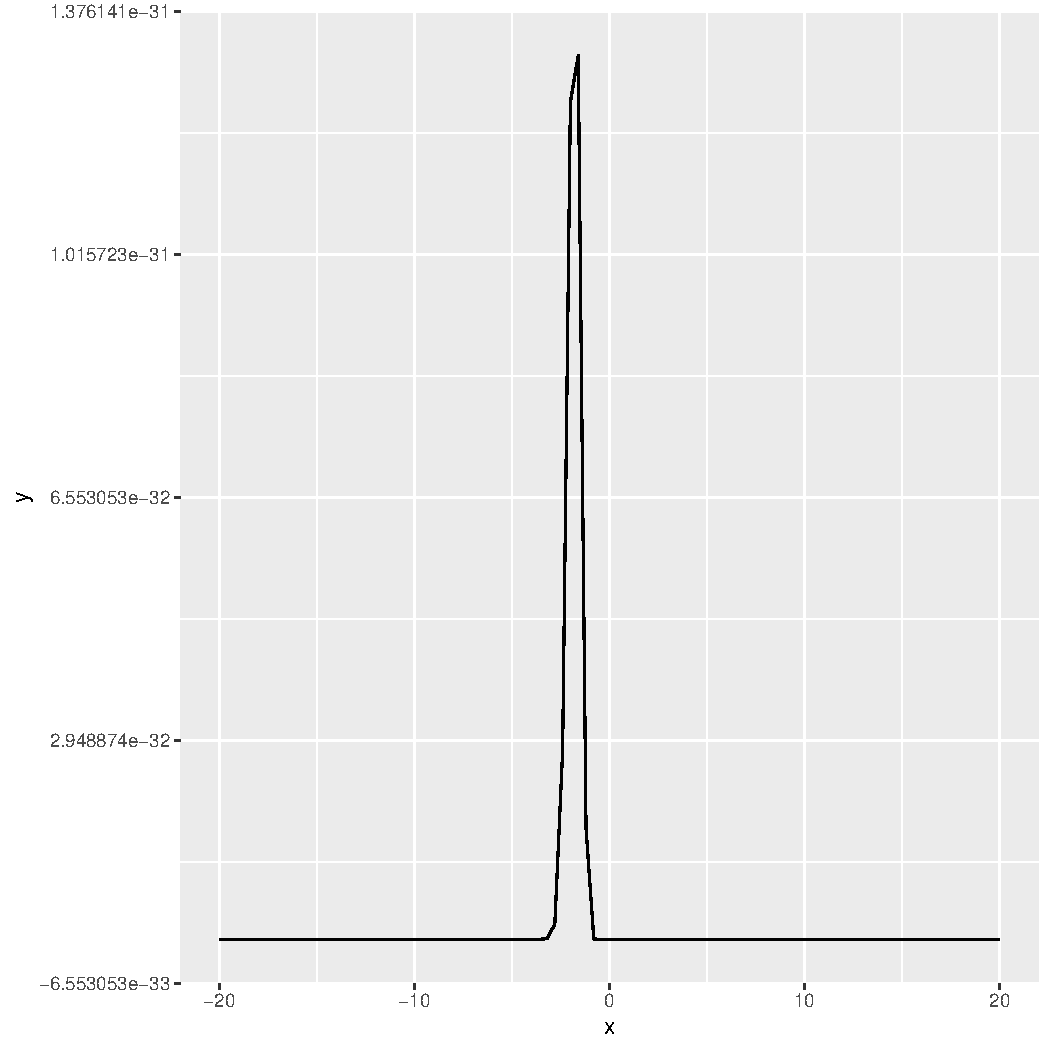
\includegraphics[width=\maxwidth]{figure/unnamed-chunk-2-1} 
\end{knitrout}
	\item
\begin{knitrout}
\definecolor{shadecolor}{rgb}{0.969, 0.969, 0.969}\color{fgcolor}\begin{kframe}
\begin{alltt}
\hldef{res} \hlkwb{=} \hlkwd{as.vector}\hldef{(}\hlkwd{resid}\hldef{(model))}
\hldef{fit} \hlkwb{=} \hlkwd{as.vector}\hldef{(}\hlkwd{fitted}\hldef{(model))}
\hldef{check} \hlkwb{=} \hldef{res} \hlopt{-} \hldef{(maxrate} \hlopt{-} \hldef{fit)}
\hldef{check} \hlcom{#which is basically all 0}
\end{alltt}
\begin{verbatim}
##  [1] -8.881784e-16  1.776357e-15 -1.332268e-15  7.105427e-15  6.217249e-15
##  [6] -2.664535e-15  8.881784e-15 -5.329071e-15 -6.217249e-15  8.881784e-15
## [11]  2.220446e-15 -6.217249e-15  1.199041e-14 -8.881784e-16  3.108624e-15
\end{verbatim}
\end{kframe}
\end{knitrout}
	from this we can conclude that \texttt{res} = \texttt{actual values} - \texttt{fit}.
	\item
\begin{knitrout}
\definecolor{shadecolor}{rgb}{0.969, 0.969, 0.969}\color{fgcolor}\begin{kframe}
\begin{alltt}
\hlkwd{predict}\hldef{(model,}\hlkwd{data.frame}\hldef{(}\hlkwc{age} \hldef{=} \hlkwd{c}\hldef{(}\hlnum{12}\hldef{,}\hlnum{33}\hldef{,}\hlnum{45}\hldef{,}\hlnum{76}\hldef{)))}
\end{alltt}
\begin{verbatim}
##        1        2        3        4 
## 200.4757 183.7235 174.1508 149.4212
\end{verbatim}
\end{kframe}
\end{knitrout}
	\item
\begin{knitrout}
\definecolor{shadecolor}{rgb}{0.969, 0.969, 0.969}\color{fgcolor}\begin{kframe}
\begin{alltt}
\hldef{test_beta1} \hlkwb{=} \hlkwa{function}\hldef{(}\hlkwc{lin_model}\hldef{,} \hlkwc{alpha} \hldef{=} \hlnum{0.05}\hldef{) \{}
        \hldef{p_val} \hlkwb{=} \hlkwd{summary}\hldef{(lin_model)}\hlopt{$}\hldef{coefficients[}\hlsng{"age"}\hldef{,} \hlsng{"Pr(>|t|)"}\hldef{]}
        \hlkwa{if}\hldef{(p_val} \hlopt{<} \hldef{alpha) \{}
                \hlkwd{return}\hldef{(}\hlsng{"Reject Null: Evidence suggests beta_1 is not 0"}\hldef{)}
        \hldef{\}} \hlkwa{else} \hldef{\{}
                \hlkwd{return}\hldef{(}\hlsng{"Fail to Reject Null"}\hldef{)}
        \hldef{\}}
\hldef{\}}
\hlkwd{test_beta1}\hldef{(model)}
\end{alltt}
\begin{verbatim}
## [1] "Reject Null: Evidence suggests beta_1 is not 0"
\end{verbatim}
\end{kframe}
\end{knitrout}
	\item
\begin{knitrout}
\definecolor{shadecolor}{rgb}{0.969, 0.969, 0.969}\color{fgcolor}\begin{kframe}
\begin{alltt}
    \hlkwd{confint}\hldef{(model,} \hlkwc{parm} \hldef{=} \hlsng{"age"}\hldef{,} \hlkwc{level} \hldef{=} \hlnum{0.95}\hldef{)}
\end{alltt}
\begin{verbatim}
##         2.5 %     97.5 %
## age -0.948872 -0.6465811
\end{verbatim}
\end{kframe}
\end{knitrout}
	\item
\begin{knitrout}
\definecolor{shadecolor}{rgb}{0.969, 0.969, 0.969}\color{fgcolor}\begin{kframe}
\begin{alltt}
\hlcom{# i. Scatter plot of residuals vs fitted values}
\hlkwd{plot}\hldef{(}\hlkwd{fitted}\hldef{(model),} \hlkwd{resid}\hldef{(model),}
\hlkwc{main}\hldef{=}\hlsng{"Residuals vs Fitted"}\hldef{)}
\hlkwd{abline}\hldef{(}\hlkwc{h}\hldef{=}\hlnum{0}\hldef{,} \hlkwc{lty}\hldef{=}\hlnum{2}\hldef{)}
\end{alltt}
\end{kframe}
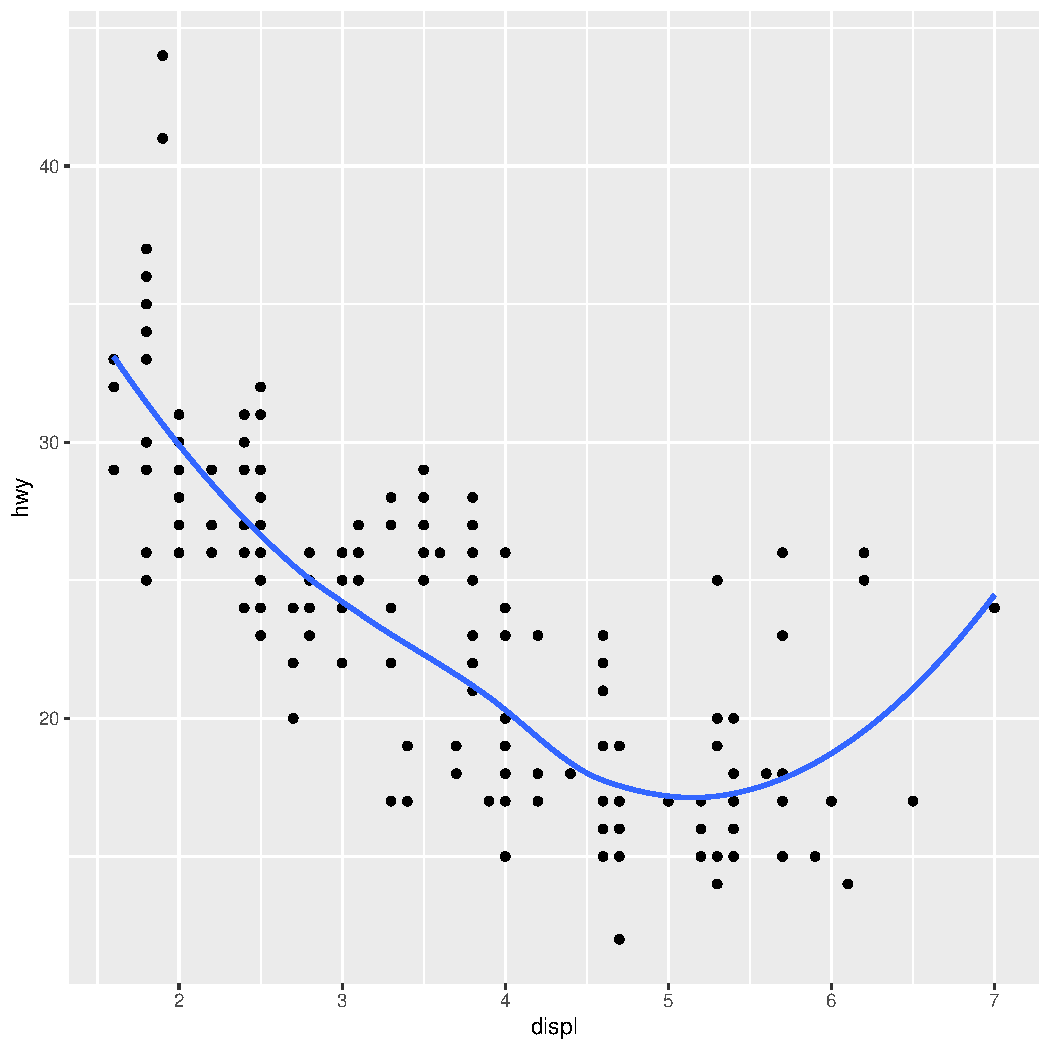
\includegraphics[width=\maxwidth]{figure/unnamed-chunk-7-1} 
\begin{kframe}\begin{alltt}
\hlcom{# ii. Scatter plot of standardized residuals vs fitted values}
\hlkwd{plot}\hldef{(}\hlkwd{fitted}\hldef{(model),} \hlkwd{sqrt}\hldef{(}\hlkwd{abs}\hldef{(}\hlkwd{rstandard}\hldef{(model))),}
\hlkwc{main}\hldef{=}\hlsng{"Std. Residuals vs Fitted"}\hldef{)}
\hlkwd{abline}\hldef{(}\hlkwc{h}\hldef{=}\hlnum{0}\hldef{,} \hlkwc{lty}\hldef{=}\hlnum{2}\hldef{)}
\end{alltt}
\end{kframe}
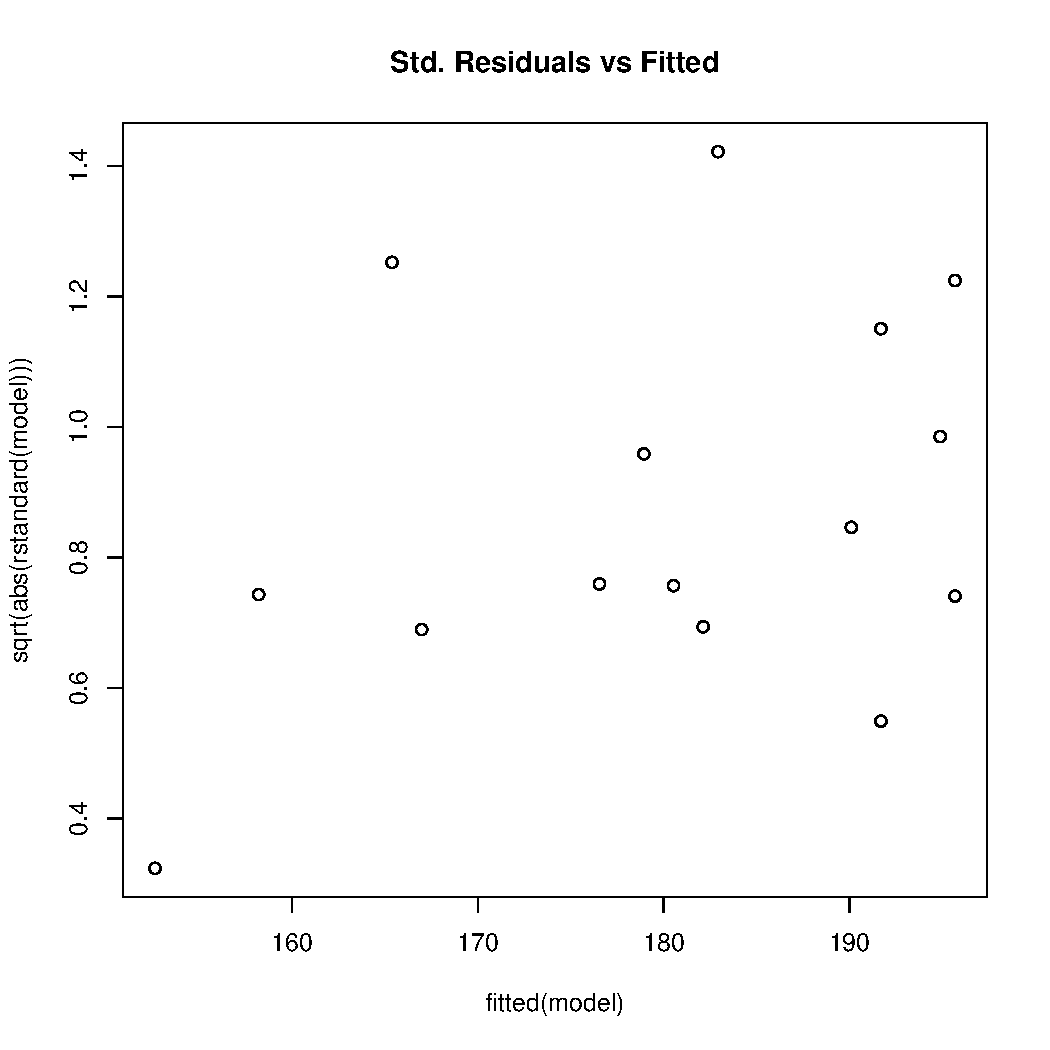
\includegraphics[width=\maxwidth]{figure/unnamed-chunk-7-2} 
\begin{kframe}\begin{alltt}
\hlcom{# iii. Normal Q-Q plot for residuals}
\hlkwd{qqnorm}\hldef{(}\hlkwd{resid}\hldef{(model))}
\hlkwd{qqline}\hldef{(}\hlkwd{resid}\hldef{(model))}
\end{alltt}
\end{kframe}
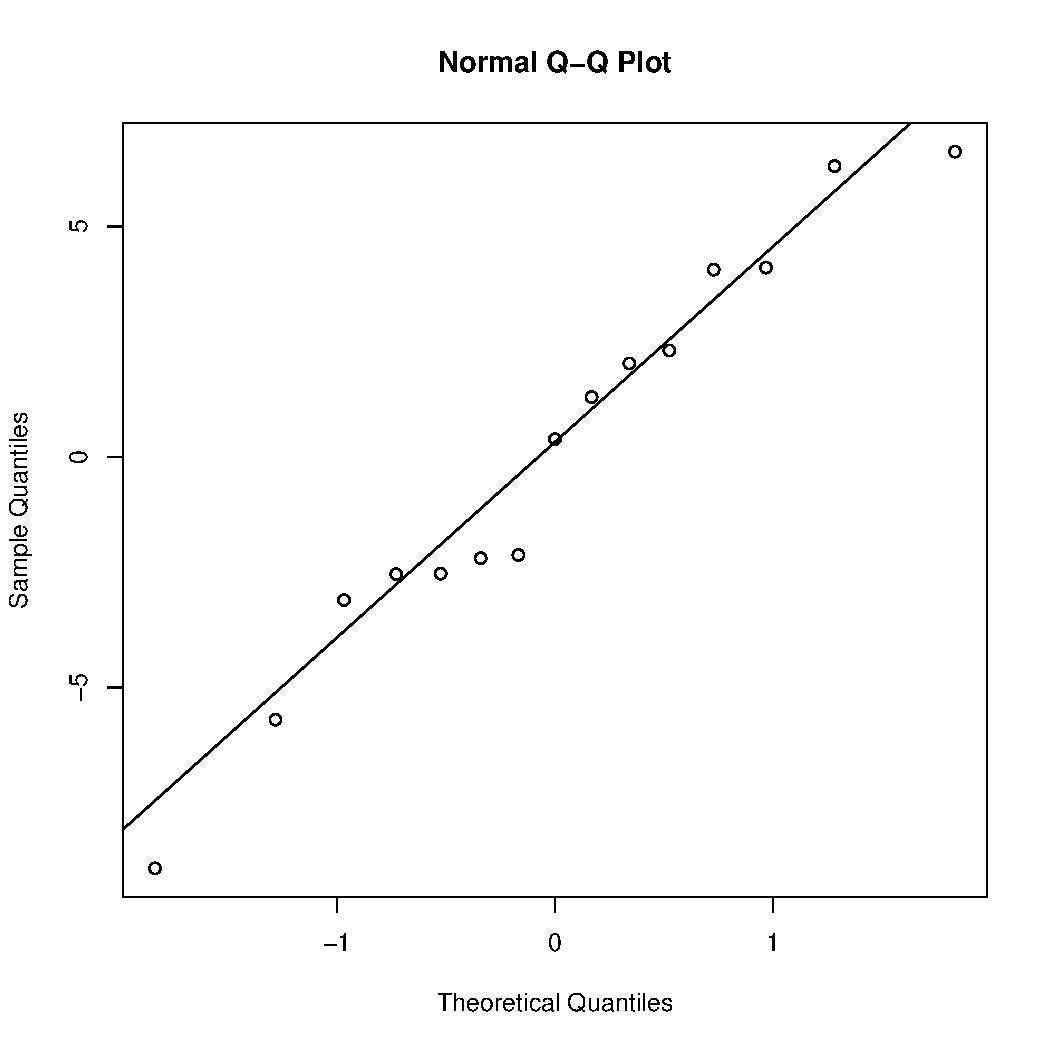
\includegraphics[width=\maxwidth]{figure/unnamed-chunk-7-3} 
\end{knitrout}
	\end{enumerate}
	\item
	\begin{enumerate}[label=(\alph*)]
	\item
\begin{knitrout}
\definecolor{shadecolor}{rgb}{0.969, 0.969, 0.969}\color{fgcolor}\begin{kframe}
\begin{alltt}
\hlkwd{cor}\hldef{(ToothGrowth}\hlopt{$}\hldef{len, ToothGrowth}\hlopt{$}\hldef{dose)}
\end{alltt}
\begin{verbatim}
## [1] 0.8026913
\end{verbatim}
\end{kframe}
\end{knitrout}
    \item
\begin{knitrout}
\definecolor{shadecolor}{rgb}{0.969, 0.969, 0.969}\color{fgcolor}\begin{kframe}
\begin{alltt}
\hlkwd{plot}\hldef{(ToothGrowth}\hlopt{$}\hldef{dose, ToothGrowth}\hlopt{$}\hldef{len,}
\hlkwc{main}\hldef{=}\hlsng{"Tooth Length vs Dose"}\hldef{,} \hlkwc{xlab}\hldef{=}\hlsng{"Dose"}\hldef{,} \hlkwc{ylab}\hldef{=}\hlsng{"Length"}\hldef{)}
\end{alltt}
\end{kframe}
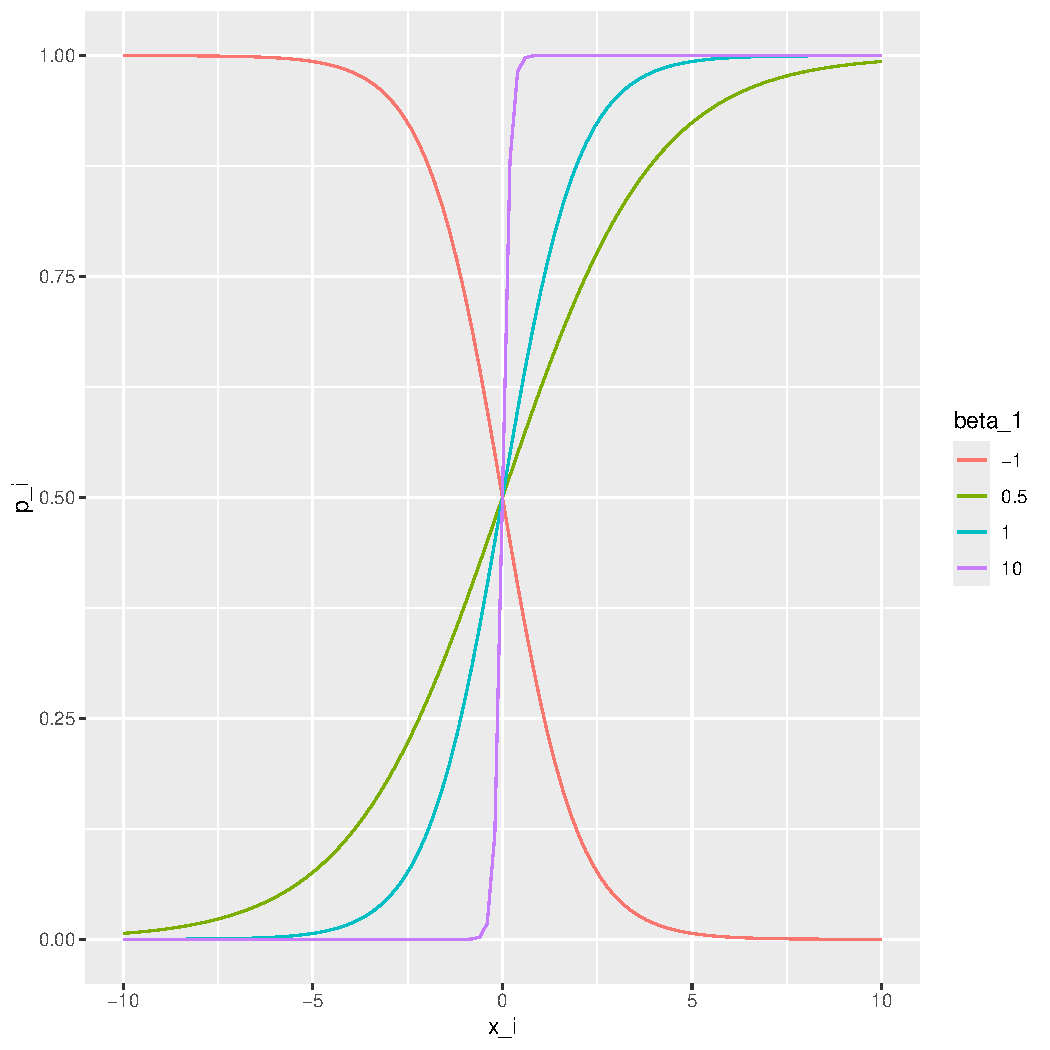
\includegraphics[width=\maxwidth]{figure/unnamed-chunk-9-1} 
\end{knitrout}
    \item
\begin{knitrout}
\definecolor{shadecolor}{rgb}{0.969, 0.969, 0.969}\color{fgcolor}\begin{kframe}
\begin{alltt}
\hldef{split_growth} \hlkwb{=} \hlkwd{split}\hldef{(ToothGrowth}\hlopt{$}\hldef{len, ToothGrowth}\hlopt{$}\hldef{dose)}
    \hldef{group_means} \hlkwb{=} \hlkwd{sapply}\hldef{(split_growth, mean)}
\hldef{group_means}
\end{alltt}
\begin{verbatim}
##    0.5      1      2 
## 10.605 19.735 26.100
\end{verbatim}
\end{kframe}
\end{knitrout}
	\item
\begin{knitrout}
\definecolor{shadecolor}{rgb}{0.969, 0.969, 0.969}\color{fgcolor}\begin{kframe}
\begin{alltt}
\hldef{doses} \hlkwb{=} \hlkwd{as.numeric}\hldef{(}\hlkwd{names}\hldef{(group_means))}
    \hlkwd{cor}\hldef{(group_means, doses)}
\end{alltt}
\begin{verbatim}
## [1] 0.9574428
\end{verbatim}
\end{kframe}
\end{knitrout}
	
	\end{enumerate}
\end{enumerate}
\end{document}
